
% \subsection{Sampling}
% Choosing samples (partition, n, scale): 
% \begin{enumerate}
%     \item compute the inverse curve, I, and std deviation for the partition. The curve is computed at n points along the $y_{min} .. y_{max}$ attained in the given partition
%     \item compute a hyper tube along the curve with hyper-rectangle cross section $\pm s \times sigma_i$ each dimension, where s is a scale given by the user 
%     \item For each of control points of the curve along y, compute the area of the cross section. Normalize by the are of the tube this defines a pdf.
%     \item select $k$ values of y using the pdf.
%     \item for each selected $y^k$ choose $x_i^k \in [I_i - s \times \sigma, I_i + s \times \sigma]$ 
% \end{enumerate}

% We run a simulation for each sample. We can use the new data in two ways. First, we can compare each proposed sample with the computed one to evaluate how well our model prediction works. In this case we can add the computed sample to the partition but not reevaluate the MSC. Second, we can restart the whole process and evaluate a new MSC and Regulus decomposition. Note that in this case, the MSC will not necessarily be the same. This is a known issue with MSC and is beyond the scope of this work. 

% \begin{figure}[thb]
%     \begin{center}
%      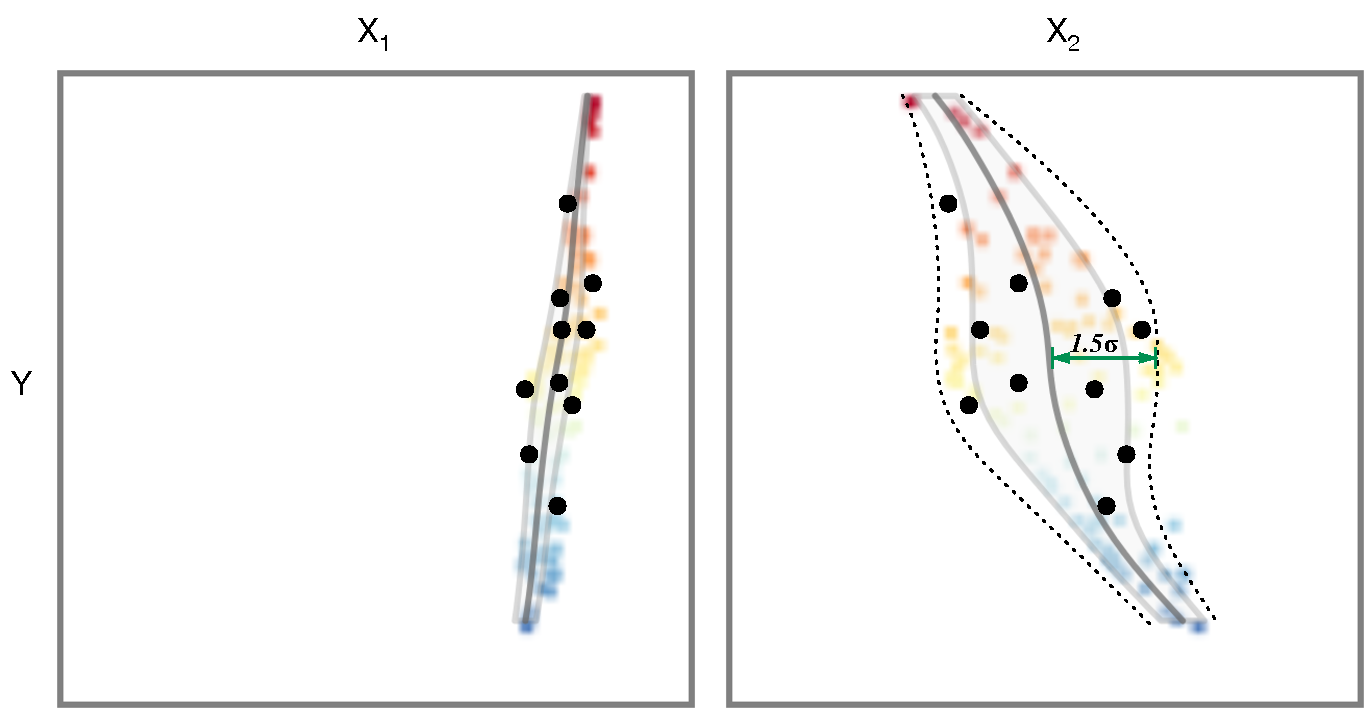
\includegraphics[width=\linewidth]{samples}
%     \caption{Selecting samples using the inverse regression curves. The inverse curve is represented by the central gray curve. The two light gray curves represent the area one $\sigma$ around the curve and the dash lines shows the sampling area defined by $s \times \sigma$ where $s$ is a scale given by the user.}
%     \label{fig:samples}
%     \end{center}
% \end{figure}